% Created 2016-12-17 Sat 16:57
\documentclass[10pt,conference,compsocconf]{IEEEtran}
\usepackage[utf8]{inputenc}
\usepackage[T1]{fontenc}
\usepackage{fixltx2e}
\usepackage{graphicx}
\usepackage{grffile}
\usepackage{longtable}
\usepackage{wrapfig}
\usepackage{rotating}
\usepackage[normalem]{ulem}
\usepackage{amsmath}
\usepackage{textcomp}
\usepackage{amssymb}
\usepackage{capt-of}
\usepackage{hyperref}
\usepackage{bm}
\usepackage{svg}
\usepackage{graphicx}
\graphicspath{{pics/}}
\usepackage[margin=1in]{geometry}
\usepackage{algorithm}
\usepackage{algpseudocode}
\graphicspath{{pics/}}
\def\arraystretch{1.7}
\documentclass[10pt,conference,compsocconf]{IEEEtran}
\author{Laurent Lejeune, Tatiana Fountoukidou, Guillaume de Montauzon}
\date{\today}
\title{Group 97: Road Segmentation}
\hypersetup{
	pdfauthor={Laurent Lejeune, Tatiana Fountoukidou, Guillaume de Montauzon},
	pdftitle={Group 97: Road Segmentation},
	pdfkeywords={},
	pdfsubject={},
	pdfcreator={Emacs 25.1.1 (Org mode 8.3.6)}, 
	pdflang={English}}
\begin{document}
	
	\maketitle
	
	\section{Introduction}
	In this project we were given a set of 100 RGB satellite images, and a corresponding binary mask for each one of them, indicating the regions of the image that represents road. Our task was, given an unknown satellite image to perform automatic segmentation of the roads, marking everything else as background. We therefore have to solve a binary classification problem, effectively for every image pixel. An example of an image and its ground truth is shown in figure~\ref{example}.
	\begin{figure}[h]
		\centering
		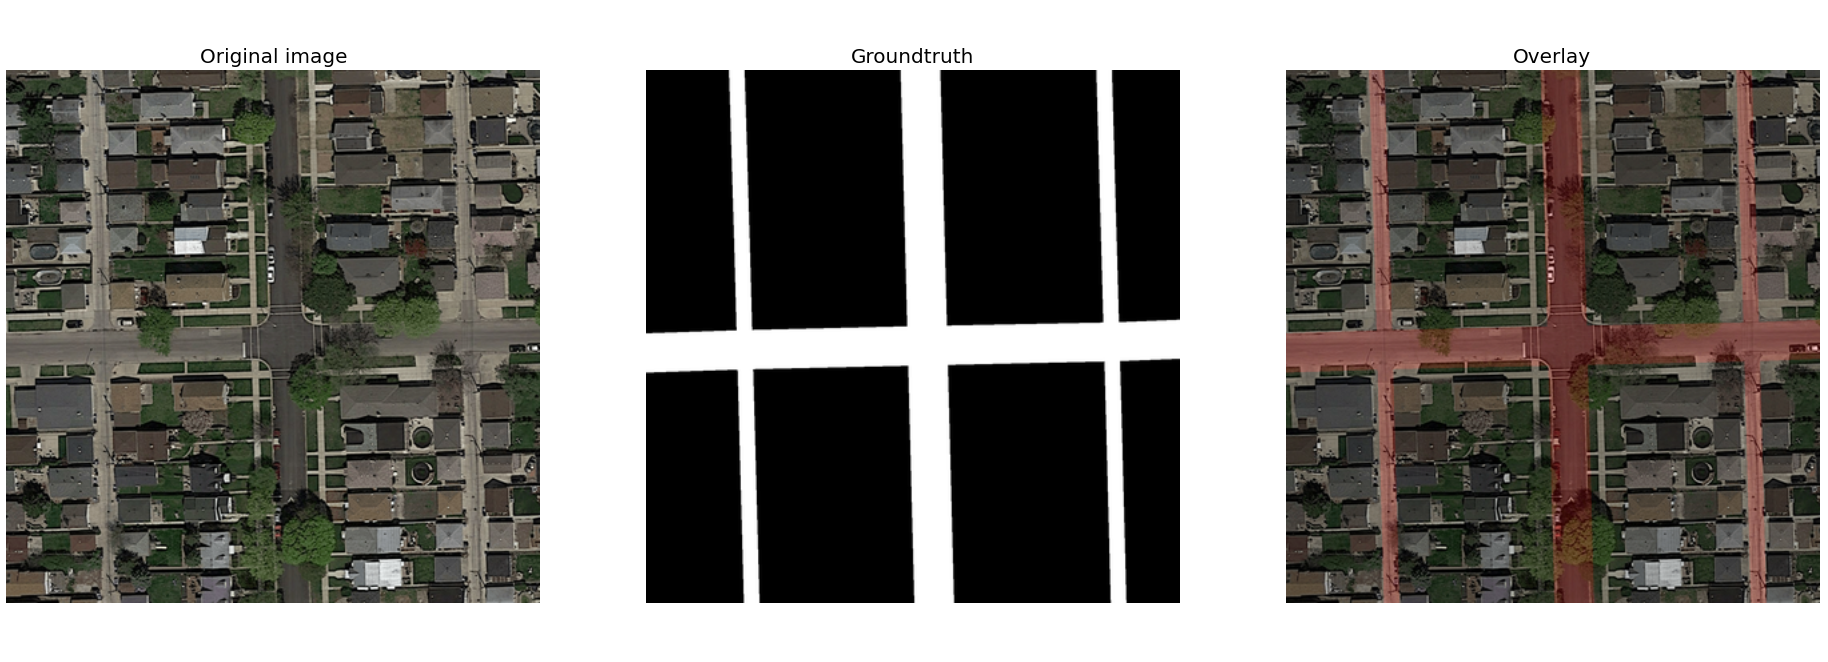
\includegraphics[width=0.5\textwidth]{example.png}
		\caption{Data example}
		\label{example}
	\end{figure}
	
%	\section{Related work}
%	\label{sec:orgheadline6}
%	\subsection{Road Segmentation in Aerial Images by Exploiting Road Vector Data \cite{6602035}}
%	\label{sec:orgheadline1}
%	\subsection{Morphological road segmentation in urban areas from high resolution satellite images \cite{gaetano:inria-00618222}}
%	\label{sec:orgheadline2}
%	\subsection{Connected Component-Based Technique for Automatic Extraction of Road Centerline in High Resolution Satellite Images \cite{sujatha15_connec_compon_based_techn_autom}}
%	\label{sec:orgheadline3}
%	\subsection{Machine Learning Based Road Detection from High Resolution Imagery}
%	\label{sec:orgheadline4}
%	\subsection{Road Extraction Using K-Means clustering and Morphological Operations \cite{maurya2011road}}
%	\label{sec:orgheadline5}
	
	\section{Baselines}
	To begin with, we set some simple baselines for tackling the problem of road segmentation. The baseline selection is described below.
	\subsection{Baseline classifier selection}
	\label{baseline_selection}
	As a baseline, every image was broken down to a number of non-overlapping $16 \times 16$ image patches. If more than 25\% of the groundtruth corresponding to the patch was road, the patch was labeled as road. This way, we ended up with a single label for every patch, thus simplifying the classification problem. As a feature, a vector of size 2 was used, containing the mean value and the variance of the pixels contained in the patch (A feature vector of size 6, consisting of the mean and the variance for each color channel was also tried, but it lead to no improvement). A grid search to indicate a simple classifier that best works for this setup was run, and the one with the best performance was set as a baseline for further improvement.	
	The performance is measured in terms of the F-score, that considers both the precision and recall, and is defined as:
	\begin{align*}
	F_1 & = 2\cdot \frac{\text{precision}\cdot \text{recall}}{\text{precision} + \text{recall}} \\
	& = 2 \cdot \frac{TP}{2TP + FN + FP}
	\end{align*}
	A 5-fold cross validation is run over the training dataset, and the F-score on the testing set is calculated for each fold. The mean and the variance of the F-score over the 5 folds is then calculated. The results of the baseline search are shown at table~\ref{baseline} (only the best parameters of each classifier are demonstrated, for clarity reasons). For the rest of the work, the performance of the random forest (RF) classifier will be used as the baseline to further investigate how these results can be improved \footnote{Note that although the RF classifier had the same performance as the SVM, the RF was significantly faster, so we decided to stick with that.}.
		\begin{table}[h]
		\centering
		\begin{tabular}{p{0.3\textwidth} c}		
			\textbf{Classifier} &  \textbf{$F_1-score (\text{mean}\pm \text{std})$}\\
			\hline \hline
			Logistic regression ($\lambda = 1e5$) & $0.44 \pm 0.02$ \\ \hline
			SVM (rbf kernel, $\lambda = 1e5$) & $0.5 \pm 0.02$ \\ \hline
			\textbf{RF (number of trees = 50, max depth = 10)} & $\bf{0.5 \pm 0.02}$ \\
			\hline
		\end{tabular}
		\label{baselines}
		\caption{Baselines}
		\end{table}
	\subsection{Patch size selection}
	We examined the impact of the patch size on the classification performance. The mean and the variance of the pixels was again used as a feature, and the classifier was the baseline RF described above. The F-score was recorded for a 5-fold cross validation, and the results for the different patch sizes are shown in table~\ref{patch_size}.
	\begin{table}[h]	
	\centering
	\begin{tabular}{lc}
		\hline \hline		
		\textbf{Patch Size} &  \textbf{F-score (mean $\pm$ std)} \\
		\hline
		8 & $0.45 \pm 0.03$ \\
		16 & $0.5 \pm 0.03$ \\
		25 & $0.54 \pm 0.04$ \\
		32 & $0.55 \pm 0.06$ \\
		\hline
	\end{tabular}
	\label{patch_size}
	\caption{Patch size comparison}
	\end{table}
	Even though the larger the patch size, the better the F-score, with a quick inspection of the data we realized that many roads were too narrow to be represented by a larger patch size. The higher score in this case is misleading, since it is calculated on a patch level, and not on a pixel level. This way, although more patches are classified correctly, the overall segmentation mask that comes up is not representative enough. For this reason, the patch size of 16 was kept, as more appropriate to capture the different road widths.
	\section{Data exploration}
	\label{sec:orgheadline7}
	The provided training set contains 100 images of size 400x400 along with their ground-truth. A total of 6 images are discarded because they either show a too small quantity of positive class pixels, or some misleading regions such as rail-tracks. 
	We notice that most images are made of grid-like roads, sometimes occluded by trees. 
	\section{Mid-level segmentations}
	\label{sec:orgheadline8}
	The image pixels are first grouped in two different manners:
	\begin{enumerate}
		\item Square patches: The image is divided in non-overlapping patches of size 16x16.
		\item SLIC Superpixels (Simple Linear Iterative Clustering) \cite{achanta12}: Pixels are grouped in mid-level regions in an iterative manner. The algorithm starts from a regular grid of cluster centers and iteratively updates the labels of their neighboring centers based on a distance measure. This method improves over the square patches method because the pixels are already pre-segmented. Their feature vector will therefore be easier to discriminate.
	\end{enumerate}
	\section{Feature extraction}
	\subsection{Features}
	\label{features}
	Following an exploration of the related litterature, we select a set of features to extract.
	\begin{itemize}
		\item SIFT (Scale-Invariant Feature Transform) \cite{lowe99}: This descriptor is used extensively in computer-vision applications. It computes a histogram of oriented gradients on 16x16 windows centered at a keypoint and gives a descriptor of 128 scalar values. The keypoint detection step is not performed, instead we extract the descriptors on a dense grid at canonical scale and orientation. As advised in \footnote{\url{https://people.csail.mit.edu/hasinoff/320/sift-notes.txt}} to improve illumination invariance, the integer value descriptors are first normalized to unit-norm, ceiled to 0.2, and renormalized to unit-norm. As we require that each segment be represented by a single feature vector, we encode the dense SIFT descriptors contained in a given segment in a "bag-of-features" manner through the following steps: 
		\begin{enumerate}
			\item Based on a sufficiently large number of SIFT descriptors computed on 10 images, we start by fitting a PCA model. We have checked that the explained variance at 60 components is above 99\%.
			\item A codebook is generated on the aforementioned training samples. A codebook is merely a set of K-means clusters that is used to encode the input (compressed) descriptors to integer values.
			\item We then compute a normalized histogram of codes (bag-of-features) in each segment. This gives us a single texture feature vector for mid-level regions.
		\end{enumerate}
		\item Hough line transform: This transformation has already been used in a state-of-the-art method \cite{2016ISPAr41B3..891L}. First, the edge map is computed using a canny edge detector. Given some parameters, a set of lines are extracted on the edge maps and sorted based on their RGB variance, i.e. we want to keep the lines along which the color variations is minimal.
		\item Euclidean distance transform. This straightforward transform is used to compute, at each pixel location, the shortest "taxicab" distance to an edge pixel. Again, a canny edge map is used as input.
	\end{itemize}
	\subsection{Refinement of generic models using Conditional Random Field}
	\label{refinement}
	Using a Conditional Random Field model, one can leverage the spatial relations between mid-level regions. Indeed, a segment considered as road gives a strong prior on the "roadness" of its neighboring segment. This is formalized as an undirected graph on which the node features are assigned unary potentials. In our case, the unary potentials are given by probability estimates given by generic models such as logistic regression or random forest.
	Inspired by \cite{fulkerson09}, the edge costs are made off of two features: The difference in mean LUV color, and the number of pixels that separate two segments (length of separating path). This last feature allows to penalize segments that are "weakly" connected. Also, we have verified visually that roads tend to be composed of regular chains of square-like segments, thereby justifying that choice.
	
	Formally, structured models aim at maximizing an energy functions of the form:
	
	\begin{equation}
	\begin{split}
	E_w(X,Y) &= \sum_{i \in \mathcal{V}} E_{data}(y_i;x_i) + \sum_{i,j \in \mathcal{E}} E_{smooth}(y_i;y_j) \\
	&= \mathbf{w}^T \psi(X,Y)
	\end{split}
	\end{equation}
	
	Where \(\mathcal{V}\) is the set of vertices representing a segment, \(\mathcal{E}\) are the edges. The data and smoothness term are combined in the joint-features vector \(\psi\). Any probabilistic regression model can be used for the data term. Following \cite{fulkerson09}, the pair-wise edges potentials are given by:
	
	\begin{equation}
	\phi(c_i,c_j|s_i,s_j) = \frac{L(s_i,s_j)}{1+\lVert s_i - s_j \rVert}
	\end{equation}
	Where \(c\) and \(s\) are the mean LUV-space colors. The function \(L\) expresses the length of the shared boundaries between two segments.
	\section{Classification}
	2 approaches were followed for this project. the first consists of feature extraction and classification, with the features mentioned aboved. The second consists of training a convolutional neural network (CNN) that takes as input the image and outputs a segmentation mask. Both approaches will be described below. 	
	
	\subsection{Classification based on feature vectors}
	The features described in~\ref{features} were used to train a random forest ensemble classifier. A grid search to define the hyperparameters of the classifier was performed. The chosen parameters were the following:
	$$\text{Number of trees} = 50$$
	$$\text{Maximum tree depth} = 10$$
	Then, the CRF refinement step described in~\ref{refinement} was also added, to see if it further improves the classification results.
	\subsection{CNNs}
	\subsubsection{Guillaume for you!!!}
	\subsubsection{U-net}
	A convolutional neural network designed for image segmentation was used, as described in~\cite{unet}. U-net is a fully convolutional neural network, meaning that it consists exclusively on convolutional and pooling layers, and not fully connected layers in the end. As a result, the output of the network is not a class assignment for the input, but a feature map. In our case the output of the network is a segmentation mask for the input image. The structure of the network is shown in figure~\ref{unet_arch}.
		\begin{figure}[h]
			\centering
			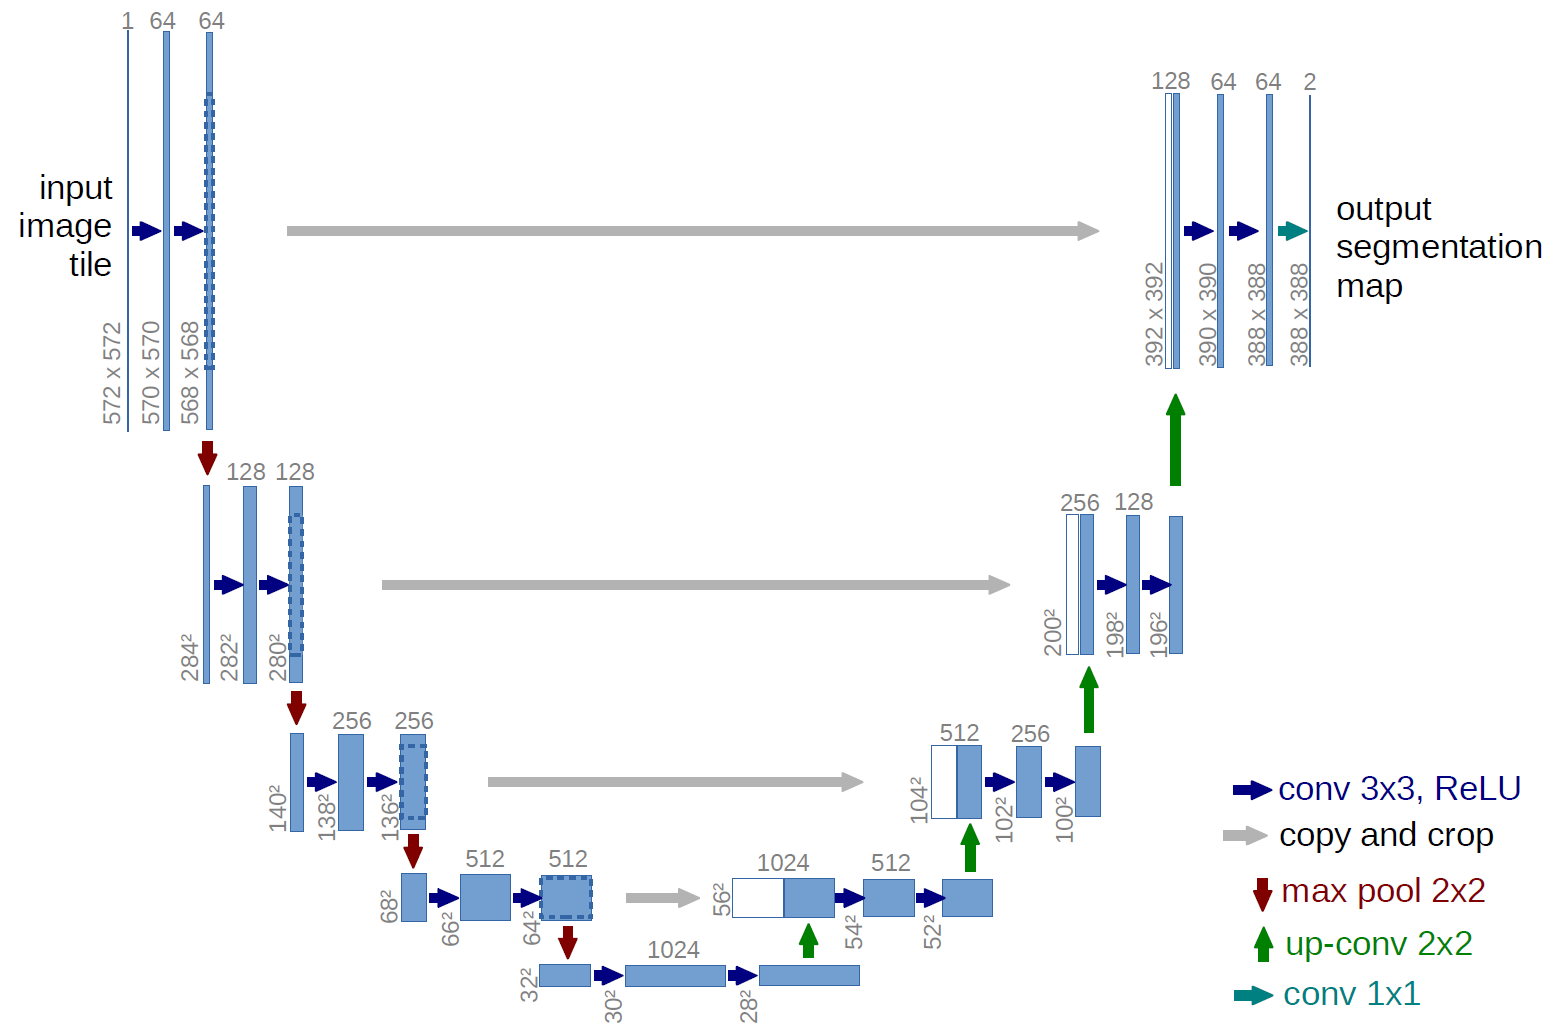
\includegraphics[width=0.5\textwidth]{unet.png}
			\caption{U-net~\cite{unet}}
			\label{unet_arch}
		\end{figure}
	\section{Results}
	The results of a 5-fold cross validation, for the different classification approaches that were attempted and described above are shown in table~\ref{results}
		\begin{table}
		\begin{tabular}{p{0.3\textwidth} c}		
			\textbf{Classification method} &  \textbf{$F_1-score (\text{mean}\pm \text{std})$}\\
			\hline \hline
			 on mean and variance features [Baseline] & $0.5 \pm 0.02$ \\ \hline
			Logistic regression with $\lambda = 1e5$ on feature vectors & $0.64 \pm 0.02$ \\ \hline
			RF on feature vectors without refinement & $0.68 \pm 0.03$ \\ \hline
			RF with CRF refinement & $0.79 \pm 0.02$ \\ \hline
			U-net & $ $ \\
			\hline
		\end{tabular}
		\label{results}
		\caption{Concentrated results}
		\end{table}
	\section{Conclusions}
	
	\label{sec:orgheadline9}
	
	
	\bibliographystyle{ieeetr}
	\bibliography{refs}
	\printbibliography
\end{document}